%iffalse
\let\negmedspace\undefined
\let\negthickspace\undefined
\documentclass[journal,12pt,onecolumn]{IEEEtran}
\usepackage{cite}
\usepackage{amsmath,amssymb,amsfonts,amsthm}
\usepackage{algorithmic}
\usepackage{graphicx}
\usepackage{textcomp}
\usepackage{xcolor}
\usepackage{txfonts}
\usepackage{listings}
\usepackage{enumitem}
\usepackage{mathtools}
\usepackage{gensymb}
\usepackage{comment}
\usepackage[breaklinks=true]{hyperref}
\usepackage{tkz-euclide} 
\usepackage{gvv}                                        
%\def\inputGnumericTable{}                                 
\usepackage[latin1]{inputenc}     
\usepackage{xparse}
\usepackage{color}                                            
\usepackage{array}                                            
\usepackage{longtable}                                       
\usepackage{calc}                                             
\usepackage{multirow}
\usepackage{multicol}
\usepackage{hhline}                                           
\usepackage{ifthen}                                           
\usepackage{lscape}
\usepackage{tabularx}
\usepackage{array}
\usepackage{float}
\newtheorem{theorem}{Theorem}[section]
\newtheorem{problem}{Problem}
\newtheorem{proposition}{Proposition}[section]
\newtheorem{lemma}{Lemma}[section]
\newtheorem{corollary}[theorem]{Corollary}
\newtheorem{example}{Example}[section]
\newtheorem{definition}[problem]{Definition}
\newcommand{\BEQA}{\begin{eqnarray}}
\newcommand{\EEQA}{\end{eqnarray}}
%\newcommand{\define}{\stackrel{\triangle}{=}}
\theoremstyle{remark}
\newtheorem{rem}{Remark}
% Marks the beginning of the document

% Marks the beginning of the document
\begin{document}
\title{CS-COMPUTER SCIENCE AND IMFORMATION TECHNOLOGY}
\author{AI25btech11022 - Narshitha}
\maketitle
\renewcommand{\thefigure}{\theenumi}
\renewcommand{\thetable}{\theenumi}
\begin {center}
\large \textbf{2011}\\


{Duration:Three hours \hfill Maximum Marks:150}
\end{center}



\begin{center}
\textbf{Q. 1 -- Q. 25 carry one mark each.}
\end{center}
\begin{enumerate}
\item In a compiler, keywords of a language are recognized during
\hfill \textbf{(GATE EE 2025)}
\begin{enumerate}
\begin{multicols}{2}
    \item parsing of the program
    \item the code generation
    \item the lexical analysis of the program
    \item dataflow analysis
    \end{multicols}
\end{enumerate}

\item A layer-4 firewall (a device that can look at all protocol headers up to the transport layer) \textbf{CANNOT}
\hfill \textbf{(GATE EE 2025)}
\begin{enumerate}
    \item block entire HTTP traffic during 9:00PM and 5:00AM
    \item block all ICMP traffic
    \item stop incoming traffic from a specific IP address but allow outgoing traffic to the same IP address
    \item block TCP traffic from a specific user on a multi-user system during 9:00PM and 5:00AM
\end{enumerate}

\item If two fair coins are flipped and at least one of the outcomes is known to be a head, what is the probability that both outcomes are heads?
\hfill \textbf{(GATE EE 2025)}
\begin{enumerate}
    \item $\frac{1}{3}$
    \item $\frac{1}{4}$
    \item $\frac{1}{2}$
    \item $\frac{2}{3}$
\end{enumerate}

\item Consider different activities related to email.
\\
m1: Send an email from a mail client to a mail server
\\
m2: Download an email from mail server to a mail client
\\
m3: Checking email in a web browser
\\
Which is the application level protocol used in each activity?\hfill \textbf{(GATE EE 2025)}
\begin{enumerate}
    \item m1: HTTP \quad m2: SMTP \quad m3: POP
    \item m1: SMTP \quad m2: FTP \quad m3: HTTP
    \item m1: SMTP \quad m2: POP \quad m3: HTTP
    \item m1: POP \quad m2: SMTP \quad m3: IMAP
\end{enumerate}

\item A company needs to develop a strategy for software product development for which it has a choice of two programming languages L1 and L2. The number of lines of code (LOC) developed using L2 is estimated to be twice the LOC developed with L1. The product will have to be maintained for five years. Various parameters for the company are given in the table below.

\begin{center}
\begin{tabular}{|l|c|c|}
\hline
\textbf{Parameter} & \textbf{Language L1} & \textbf{Language L2} \\ \hline
Man years needed for development & LOC/10000 & LOC/10000 \\ \hline

Maintenance time & 5 years & 5 years \\ \hline

\end{tabular}
\end{center}

Total cost of the project includes cost of development and maintenance. What is the LOC for L1 for which the cost of the project using L1 is equal to the cost of the project using L2?\hfill \textbf{(GATE EE 2025)}
\begin{enumerate}
    \item 4000
    \item 5000
    \item 4333
    \item 4667
\end{enumerate}

\item Let the time taken to switch between user and kernel modes of execution be $t_1$, while the time taken to switch between two processes be $t_2$. Which of the following is \textbf{TRUE}?\hfill \textbf{(GATE EE 2025)}
\begin{enumerate}
    \item $t_1 > t_2$
    \item $t_1 = t_2$
    \item $t_1 < t_2$
    \item nothing can be said about the relation between $t_1$ and $t_2$
\end{enumerate}

\item A company needs to develop digital signal processing software for one of its newest inventions. The software is expected to have 40000 lines of code. The company needs to determine the effort in person-months needed to develop this software using the basic COCOMO model. The multiplicative factor for this model is given as 2.8 for the software development on embedded systems, while the exponentiation factor is given as 1.20. What is the estimated effort in person-months?\hfill \textbf{(GATE EE 2025)}
\begin{enumerate}
    \item 234.25
    \item 932.50
    \item 287.80
    \item 122.40
\end{enumerate}

\item Which of the following pairs have \textbf{DIFFERENT} expressive power?\hfill \textbf{(GATE EE 2025)}
\begin{enumerate}
    \item Deterministic finite automata (DFA) and Non-deterministic finite automata (NFA)
    \item Deterministic push down automata (DPDA) and Non-deterministic push down automata (NPDA)
    \item Deterministic single-tape Turing machine and Non-deterministic single-tape Turing machine
    \item Single-tape Turing machine and multi-tape turing machine
\end{enumerate}


\item  HTML (HyperText Markup Language) has language elements which permit certain actions other than describing the structure of the web document. Which one of the following actions is \textbf{NOT} supported by pure HTML (without any server or client side scripting) pages?\hfill \textbf{(GATE EE 2025)}

\begin{enumerate}
\item Embed web objects from different sites into the same page
\item Refresh the page automatically after a specified interval
\item Automatically redirect to another page upon download
\item Display the client time as part of the page
\end{enumerate}


\item  Which one of the following is \textbf{NOT} desired in a good Software Requirement Specifications (SRS) document?\hfill \textbf{(GATE EE 2025)}

\begin{enumerate}
\item Functional Requirements
\item Non-Functional Requirements
\item Goals of Implementation
\item Algorithms for Software Implementation
\end{enumerate}


\item A computer handles several interrupt sources, which of the following are relevant for this question:

 Interrupt from CPU temperature sensor (raises interrupt if CPU temperature is too high)
\\
     Interrupt from Mouse (raises interrupt if the mouse is moved or a button is pressed)
     \\
    Interrupt from Keyboard (raises interrupt when key is pressed or released)
    \\
Interrupt from Hard Disk (raises interrupt when a disk read is completed)
\\
  Which one of these will be handled at the \textbf{HIGHEST} priority?
  \hfill \textbf{(GATE EE 2025)}
\begin{enumerate}
\item  Interrupt from Hard Disk
\item   Interrupt from Mouse
\item   Interrupt from Keyboard
\item   Interrupt from CPU temperature sensor
\end{enumerate}


\item Consider a relational table with a single record for each registered student with the following attributes
\\
1. Registration\_Nam: Unique registration number of each registered student
\\
2. UID: Unique identity number ,unique at national level for each citizen 
\\
3.BankAccount\_Num:Unique account number at bank
\\
4. Name:name of the student 
\\
5. Hostel\_Room: Room number of the hostel 
\\
Which of the following is \textbf{INCORRECT ?}\hfill \textbf{(GATE EE 2025)}
\begin{enumerate}
    \item BankAccount\_Num is a candidiate key
    \item Registration\_Num  can be a primary key 
    \item UID is a candidiate key if all the students are from same country
    \item If S is a superkey such that $S\cap UID$ is NULL then $S\cap UID$ is also a superkey
\end{enumerate}
\item Which one of the following circuits is \textbf{NOT} equivalent to a 2-input XNOR \brak{exclusive NOR} gate? \hfill \textbf{(GATE EE 2025)}
\begin{figure}[h]
    \centering
    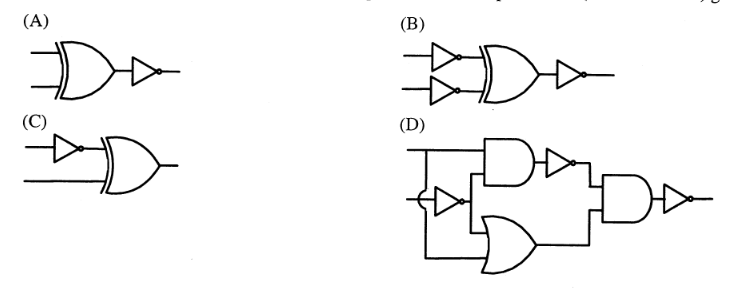
\includegraphics[width=0.9\linewidth]{figs/fig1.png}
    \caption{ }
    \label{fig1}
\end{figure}


\item The simplified SOP (Sum of Products) form of the Boolean expression
\[
    (P + \overline{Q} + R) \cdot (P + \overline{Q} + \overline{R}) \cdot (P + Q + \overline{R})
\]
is \hfill \textbf{(GATE EE 2025)}
\begin{enumerate}
\begin{multicols}{2}
\item $(\overline{P}Q + \overline{R})$
\item $(P + \overline{Q}\,\overline{R})$
\item $(\overline{P}Q + R)$
\item $(P Q + R)$
\end{multicols}
\end{enumerate}


\item  The minimum number of D flip-flops needed to design a mod-258 counter is: \hfill \textbf{(GATE EE 2025)}
\begin{enumerate}
\begin{multicols}{4}
\item  $9$
\item   $8$
\item   $512$
\item   $258$
\end{multicols}
\end{enumerate}



\item  A thread is usually defined as a ``light weight process'' because an operating system (OS) maintains smaller data structures for a thread than for a process. In relation to this, which of the following is \textbf{TRUE}? \hfill \textbf{(GATE EE 2025)}
\begin{enumerate}
\item  On per-thread basis, the OS maintains \textit{only} CPU register state
\item   The OS does not maintain a separate stack for each thread
\item   On per-thread basis, the OS does not maintain virtual memory state
\item   On per-thread basis, the OS maintains \textit{only} scheduling and accounting information
\end{enumerate}




\item K4 and Q3 are graphs with the following structures.
\\
Which one of the following statements is TRUE in relation to these graphs? \hfill \textbf{(GATE EE 2025)}
\begin{figure}
    \centering
    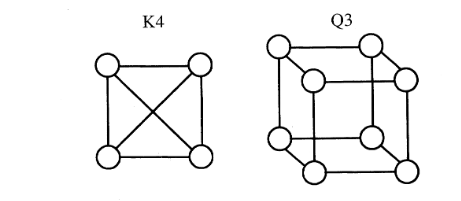
\includegraphics[width=0.5\linewidth]{figs/fig2.png}
    \caption{Caption}
    \label{fig:placeholder}
\end{figure}
\begin{enumerate}
  \item K4 is planar while Q3 is not
  \item Both K4 and Q3 are planar
  \item Q3 is planar while K3 is not
  \item  Neither K4 nor Q3 is planar
\end{enumerate}


\item If the difference between the expectation of the square of a random variable $ E[X^2] $ and the square of the expectation of the random variable $ (E[X])^2 $ is denoted by $ R $, then \hfill \textbf{(GATE EE 2025)}

\begin{enumerate}
  \item $ R = 0 $
  \item $ R < 0 $
  \item $ R \geq 0 $
  \item $ R > 0 $
\end{enumerate}


\item The lexical analysis for a modern computer language such as Java needs the power of which one of the following machine models in a necessary and sufficient sense? \hfill \textbf{(GATE EE 2025)}

\begin{enumerate}
  \item Finite state automata
  \item Deterministic pushdown automata
  \item Non-deterministic pushdown automata
  \item Turing machine
\end{enumerate}




\item Let the page fault service time be 10 ms in a computer with average memory access time being 20 ns. If one page fault is generated for every $ 10^6 $ memory accesses, what is the effective access time for the memory? \hfill \textbf{(GATE EE 2025)}

\begin{enumerate}
  \item 21 ns
  \item  30 ns
  \item 23 ns
  \item 35 ns
\end{enumerate}




\item Consider a hypothetical processor with an instruction of type \texttt{LW R1, 20(R2)}, which during execution reads a 32-bit word from memory and stores it in a 32-bit register R1. The effective address of the memory location is obtained by the addition of a constant 20 and the contents of register R2. Which of the following best reflects the addressing mode implemented by this instruction for the operand in memory? \hfill \textbf{(GATE EE 2025)}

\begin{enumerate}
  \item Immediate Addressing
  \item Register Addressing
  \item Register Indirect Scaled Addressing
  \item Base Indexed Addressing
\end{enumerate}


\item What does the following fragment of C program print?

\begin{lstlisting}[language=C]
char c[] = "GATE2011";
char *p = c;
printf("%s", p + p[3] - p[1]);
\end{lstlisting}
\hfill \textbf{(GATE EE 2025)}
\begin{enumerate}
  \item GATE2011
  \item E2011
  \item 2011
  \item 011
\end{enumerate}
\item A max-heap is a heap where the value of each parent is greater than or equal to the value of its children. Which of the following is a max-heap ? \hfill \textbf{(GATE EE 2025)}
\begin{figure}[h]
    \centering
    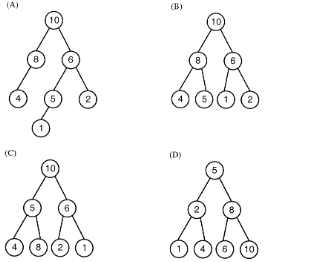
\includegraphics[width=0.5\linewidth]{figs/fig3.png}
    \caption{ }
    \label{fig3}
\end{figure}

\item Let $ P $ be a regular language and $ Q $ be a context-free language such that $ Q \subseteq P $. (For example, let $ P $ be the language represented by the regular expression $ p^* $ and $ Q = \{p^n \mid n \in \mathbb{N}\} $). Then which of the following is \textbf{ALWAYS} regular? \hfill \textbf{(GATE EE 2025)}

\begin{enumerate}
    \item $ P \cap Q $
    \item $ P - Q $
    \item $ \Sigma^* - P $
    \item $ \Sigma^* - Q $
\end{enumerate}



\item An algorithm is to find the length of the longest monotonically increasing sequence of numbers in an array $ A[0: n-1] $ is given below.

Let $ L_i $ denote the length of the longest monotonically increasing sequence starting at index $ i $ in the array.

For all $ i $ such that $ 0 \leq i \leq n - 2 $,


\[
L_i = 
\begin{cases} 
1 + L_{i+1} & \text{if } A[i] < A[i+1] \\
1 & \text{Otherwise}
\end{cases}
\]



Finally, the length of the longest monotonically increasing sequence is $ \max (L_0, L_1, \ldots, L_{n-1}) $.

Which of the following statements is \textbf{TRUE}? \hfill \textbf{(GATE EE 2025)}

\begin{enumerate}
    \item The algorithm uses dynamic programming paradigm
    \item The algorithm has a linear complexity and uses branch and bound paradigm
    \item The algorithm has a linear and non-polynomial complexity and uses branch and bound paradigm
    \item The algorithm uses divide and conquer paradigm
\end{enumerate}



\item  Consider the languages $ L_1 $, $ L_2 $, and $ L_3 $ as given below.



\[
L_1 = \{0^n1^n \mid p, q \in \mathbb{N}\}
\]




\[
L_2 = \{0^p1^q \mid p, q \in \mathbb{N} \text{ and } p = q\}
\]




\[
L_3 = \{0^p1^q \mid p, q \in \mathbb{N} \text{ and } p \neq q\}
\]


 Which of the following statements is \textbf{NOT TRUE}?
\hfill \textbf{(GATE EE 2025)}




\begin{enumerate}
    \item Push Down Automata (PDA) can be used to recognize $ L_1 $ and $ L_2 $
    \item $ L_1 $ is a regular language
    \item All the three languages are context-free
    \item Turing machines can be used to recognize all the languages
\end{enumerate}



\item Consider two binary operators '$ \uparrow $' and '$ \downarrow $' with the precedence of operator '$ \downarrow $' being lower than that of the operator '$ \uparrow $'. Operator '$ \uparrow $' is \textbf{right associative} while operator '$ \downarrow $' is \textbf{left associative}.

Which one of the following represents the parse tree for expression $ (7 \downarrow 3 \uparrow 1) \uparrow (3 \downarrow 2) $? \hfill \textbf{(GATE EE 2025)}
\begin{figure}[h]
    \centering
    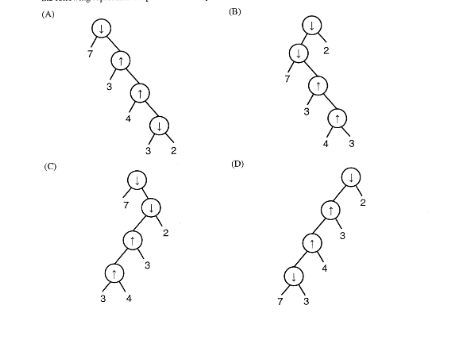
\includegraphics[width=0.5\linewidth]{figs/fig4.png}
    \caption{ }
    \label{fig4}
\end{figure}

\item On a non-pipelined sequential processor, a program segment, which is a part of the interrupt service routine, is given to transfer 500 bytes from an I/O device to memory. 

\begin{verbatim}
    Initialize the address register
    Initialize the count to 500
LOOP: Load a byte from device
      Store in memory at address given by address register
      Increment the address register
      Decrement the count
      If count != 0 go to LOOP
\end{verbatim}

Assume that each statement in this program is equivalent to a machine instruction which takes one clock cycle to execute if it is a non-load/store instruction. The load-store instructions take two clock cycles to execute.  

The designer of the system also has an alternate approach of using the DMA controller to implement the same transfer. The DMA controller requires 20 clock cycles for initialization and other overheads. Each DMA transfer cycle takes two clock cycles to transfer one byte of data from the device to the memory.  

What is the approximate speedup when the DMA controller based design is used in place of the interrupt driven program based input-output?  \hfill \textbf{(GATE EE 2025)}

\begin{enumerate}
\begin{multicols}{4}
\item 3.4  
\item 4.4 
\item  5.1 
\item  6.7
\end{multicols}
\end{enumerate}



\item We are given a set of $n$ distinct elements and an unlabeled binary tree with $n$ nodes. In how many ways can we populate the tree with the given set so that it becomes a binary search tree?  \hfill \textbf{(GATE EE 2025)}

\begin{enumerate}
\begin{multicols}{4}
\item  0 
\item 1 
\item  n! 
\item $\binom{2n-2}{n-1}$
\end{multicols}
\end{enumerate}

---

\item Which one of the following options is CORRECT given three positive integers $x, y$ and $z$, and a predicate  

\[
P(x) = (\neg(x=1) \wedge \forall y (\exists z (x = y \cdot z) \Rightarrow (y = x) \vee (y=1)))
\]
\hfill \textbf{(GATE EE 2025)}
\begin{enumerate}
\item  P(x) \text{ being true means that } x \text{ is a prime number}

\item  P(x) \text{ being true means that } x \text{ is a number other than 1}


\item  P(x) \text{ is always true irrespective of the value of } x

\item  P(x) \text{ being true means that } x \text{ has exactly two factors other than 1 and } x


\end{enumerate}


\item Given $i = \sqrt{-1}$, what will be the evaluation of the definite integral  

\[
\int_{0}^{2\pi} \frac{\cos x + i \sin x}{\cos x - i \sin x} \, dx ?
\]
\hfill \textbf{(GATE EE 2025)}
\begin{enumerate}
\begin{multicols}{4}
\item  0  
\item  2 
\item  -i 
\item i
\end{multicols}
\end{enumerate}





\item Consider a database table $T$ containing two columns $X$ and $Y$ each of type \texttt{integer}. After the creation of the table, one record $(X=1, Y=1)$ is inserted in the table.  

Let $MX$ and $MY$ denote the respective maximum values of $X$ and $Y$ among all records in the table at any point in time. Using $MX$ and $MY$, new records are inserted in the table 128 times with $X$ and $Y$ values being $MX+1, 2 \cdot MY+1$ respectively. It may be noted that each time after the insertion, values of $MX$ and $MY$ change.  

What will be the output of the following SQL query after the steps mentioned above are carried out?  \hfill \textbf{(GATE EE 2025)}

\begin{verbatim}
SELECT Y FROM T WHERE X=7;
\end{verbatim}

\begin{enumerate}
\begin{multicols}{4}
\item 127  
\item  255 
\item  129 
\item  257
\end{multicols}
\end{enumerate}




\item Consider a finite sequence of random values $X = [x_1, x_2, \ldots, x_n]$. Let $\mu_x$ be the mean and $\sigma_x$ be the standard deviation of $X$. Let another finite sequence $Y$ of equal length be derived from this as $y_i = a x_i + b$, where $a$ and $b$ are positive constants. Let $\mu_y$ be the mean and $\sigma_y$ be the standard deviation of this sequence. Which one of the following statements is \textbf{INCORRECT}?
\hfill \textbf{(GATE EE 2025)}
\begin{enumerate}
    \item Index position of mode of $X$ in $X$ is the same as the index position of mode of $Y$ in $Y$.
    \item Index position of median of $X$ in $X$ is the same as the index position of median of $Y$ in $Y$.
    \item $\mu_y = a \mu_x + b$
    \item $\sigma_y = a \sigma_x + b$
\end{enumerate}


\item A deck of $5$ cards (each carrying a distinct number from $1$ to $5$) is shuffled thoroughly. Two cards are then removed one at a time from the deck. What is the probability that the two cards are selected with the number on the first card being one higher than the number on the second card?
\hfill \textbf{(GATE EE 2025)}
\begin{enumerate}
\begin{multicols}{4}
    \item $1/5$
    \item $4/25$
    \item $1/4$
    \item $2/5$
    \end{multicols}
\end{enumerate}


\item Consider the following table of arrival time and burst time for three processes P0, P1 and P2.

\[
\begin{array}{|c|c|c|}
\hline
\text{Process} & \text{Arrival time (ms)} & \text{Burst time (ms)} \\
\hline
P0 & 0 & 8 \\
P1 & 1 & 4 \\
P2 & 2 & 9 \\
\hline
\end{array}
\]

The pre-emptive shortest job first scheduling algorithm is used. Scheduling is carried out only at arrival or completion of processes. What is the average waiting time for the three processes?
\hfill \textbf{(GATE EE 2025)}
\begin{enumerate}
\begin{multicols}{4}
    \item 5.0 ms
    \item 4.33 ms
    \item 6.33 ms
    \item 7.33 ms
    \end{multicols}
\end{enumerate}


\item Consider evaluating the following expression tree on a machine with load-store architecture in which memory can be accessed only through load and store instructions. The variables a, b, c, d are initially stored in memory. The binary operators used in this expression tree can be evaluated by the machine only when the operands are in registers. The instructions produce results only in a register. If no intermediate results can be stored in memory, what is the minimum number of registers needed to evaluate this expression? \hfill \textbf{(GATE EE 2025)}
\begin{figure}
    \centering
    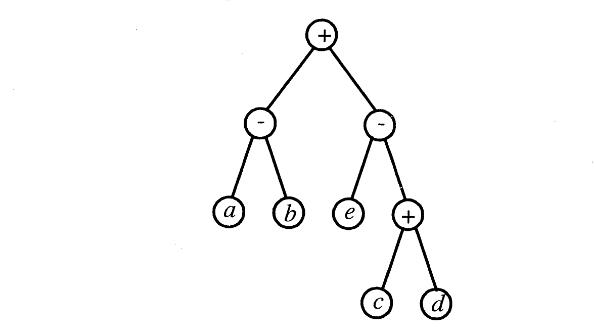
\includegraphics[width=0.5\linewidth]{figs/fig5.png}
    \caption{}
    \label{fig5}
\end{figure}

\begin{enumerate}
\begin{multicols}{4}
    \item 2
    \item 9
    \item 5
    \item 3
    \end{multicols}
\end{enumerate}


\item Which of the given options provides the increasing order of asymptotic complexity of functions $f_1, f_2, f_3$ and $f_4$?

\[
f_1(n) = 2^n, \quad f_2(n) = n^{3/2}, \quad f_3(n) = n \log n, \quad f_4(n) = n^{\log_2 n}
\]
\hfill \textbf{(GATE EE 2025)}
\begin{enumerate}
\begin{multicols}{2}
    \item $f_3, f_2, f_4, f_1$
    \item $f_2, f_3, f_4, f_1$
    \item $f_2, f_3, f_1, f_4$
    \item $f_3, f_2, f_1, f_4$
    \end{multicols}
\end{enumerate}


\item Four matrices $M_1, M_2, M_3$ and $M_4$ of dimensions $p \times q, \; q \times r, \; r \times s, \; s \times t$ respectively can be multiplied in several ways with different number of total scalar multiplications. For example when multiplied as $(((M_1 M_2) M_3) M_4)$, the total number of scalar multiplications is $pqr + prs + pst$. When multiplied as $((M_1 (M_2 M_3)) M_4)$, the total number of scalar multiplications is $pqr + rst + prt$. What is the minimum number of scalar multiplications needed if

\[
p = 10, \; q = 100, \; r = 20, \; s = 5, \; t = 80 ?
\]
\hfill \textbf{(GATE EE 2025)}
\begin{enumerate}
\begin{multicols}{4}
    \item 248000
    \item 44000
    \item 19000
    \item 25000
    \end{multicols}
\end{enumerate}


\item Consider a relational table $r$ with sufficient number of records, having attributes $A_1, A_2, \ldots, A_n$ and let $1 \leq p \leq n$. Two queries Q1 and Q2 are given below.

\[
\text{Q1: } \pi_{A_1,\ldots,A_p} \big( \sigma_{A_{p} = c}(r) \big) \quad \text{where $c$ is a constant}
\]
\[
\text{Q2: } \pi_{A_1,\ldots,A_p} \big( \sigma_{c_1 \leq A_{p} \leq c_2}(r) \big) \quad \text{where $c_1$ and $c_2$ are constants}
\]

The database can be configured to do ordered indexing on $A_p$ or hashing on $A_p$. Which of the following statements is \textbf{TRUE}?
\hfill \textbf{(GATE EE 2025)}
\begin{enumerate}
    \item Ordered indexing will always outperform hashing for both queries.
    \item Hashing will always outperform ordered indexing for both queries.
    \item Hashing will outperform ordered indexing on Q1, but not on Q2.
    \item Hashing will outperform ordered indexing on Q2, but not on Q1.
\end{enumerate}


\item  Consider the matrix as given below.
\begin{align}
    \myvec{1 & 2 & 3\\ 0 & 4 & 7\\0 & 0 & 3\\}
\end{align}

Which one of the following options provides the \textbf{CORRECT} values of the eigenvalues of the matrix? \hfill \textbf{(GATE EE 2025)} 

\begin{enumerate}
\begin{multicols}{4}
\item 1, 4, 3
\item 3, 7, 3
\item 7, 3, 2
\item 1, 2, 3
\end{multicols}
\end{enumerate}


\item  Consider an instruction pipeline with four stages (S1, S2, S3 and S4) each with combinational circuit only. The pipeline registers are required between each stage and at the end of the last stage. Delays for the stages and for the pipeline registers are as given in the figure.  
\begin{figure}
    \centering
    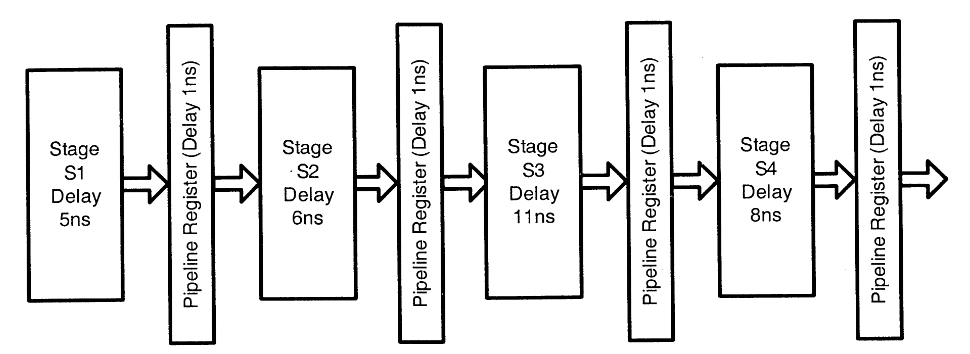
\includegraphics[width=0.5\linewidth]{figs/fig6.png}
    \caption{}
    \label{fig6}
\end{figure}


What is the approximate speed up of the pipeline in steady state under ideal conditions when compared to the corresponding non-pipeline implementation? \hfill \textbf{(GATE EE 2025)} 

\begin{enumerate}
\begin{multicols}{4}
\item 4.0
\item 2.25
\item 1.1
\item 3.0
\end{multicols}
\end{enumerate}


\item  Definition of a language \textbf{L} with alphabet \(\{a\}\) is given as follows:

$L = \{ a^{k} \mid k > 0, \; k \text{ is a positive integer constant} $

What is the minimum number of states needed in a DFA to recognize \(L\)? \hfill \textbf{(GATE EE 2025)} 

\begin{enumerate}
\begin{multicols}{4}
\item $k+1$
\item $n+1$
\item $2^{k+1}$
\item $2^{n+1}$
\end{multicols}
\end{enumerate}

\item  An 8KB direct-mapped write-back cache is organized as multiple blocks, each of size 32 bytes. The processor generates 32-bit addresses. The cache controller maintains the tag information for each cache block comprising of the following:



What is the total size of memory needed at the cache controller to store meta-data (tags) for the cache?\hfill \textbf{(GATE EE 2025)} 

\begin{enumerate}
\begin{multicols}{4}
\item 4864 bits
\item 6144 bits
\item 6656 bits
\item 5376 bits
\end{multicols}
\end{enumerate}


\item  An application loads 100 libraries at startup. Loading each library requires exactly one disk access. The seek time of the disk to a random location is given as 10 ms. Rotational speed of disk is 6000 rpm. Transfer rate of disk is 4 MB/s. Assume that average seek time and rotational latency are incurred only once, and all 100 libraries are loaded from random locations on the disk. How long will it take to load all libraries? (The time to transfer data from the disk block once the head has been positioned at the start of the block may be neglected.) \hfill \textbf{(GATE EE 2025)}

\begin{enumerate}
\begin{multicols}{4}
\item 0.50 s
\item 1.50 s
\item 1.25 s
\item 1.00 s
\end{multicols}
\end{enumerate}


\item  A deterministic finite automaton (DFA) \(D\) with alphabet \(\Sigma = \{a, b\}\) is given below.  \hfill \textbf{(GATE EE 2025)}
\begin{figure}[h]
    \centering
    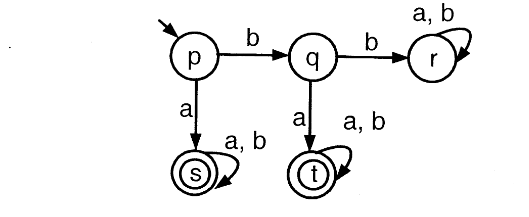
\includegraphics[width=0.5\linewidth]{figs/fig7.png}
    \caption{ }
    \label{fig7}
\end{figure}

Which of the following finite state machines is a valid minimal DFA which accepts the same language as \textbf{D}? \hfill \textbf{(GATE EE 2025)}
\begin{figure}[H]
    \centering
    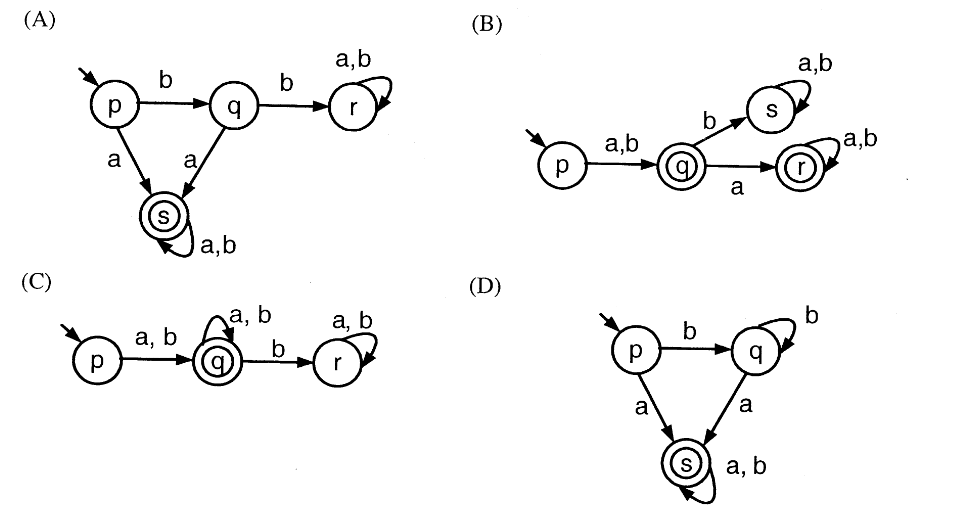
\includegraphics[width=0.5\linewidth]{figs/fig8.png}
    \caption{}
    \label{fig8}
\end{figure}

\item  Database table by name \texttt{Loan\_Records} is given below. \hfill \textbf{(GATE EE 2025)}  

\begin{center}
\begin{tabular}{|c|c|c|}
\hline
\textbf{Borrower} & \textbf{Bank\_Manager} & \textbf{Loan\_Amount} \\
\hline
Ramesh & Sundergarjan & 10000.00 \\ \hline
Suresh & Ramgopal & 5000.00 \\ \hline
Mahesh & Sundergarjan & 7000.00 \\ 
\hline
\end{tabular}
\end{center}

What is the output of the following SQL query?

\begin{verbatim}
SELECT count(*)
FROM (
    (SELECT Borrower, Bank_Manager FROM Loan_Records) AS S
    NATURAL JOIN
    (SELECT Bank_Manager, Loan_Amount FROM Loan_Records) AS T
);
\end{verbatim}

\begin{enumerate}
\begin{multicols}{4}
\item 3
\item 9
\item 5
\item 6
\end{multicols}
\end{enumerate}
\item  The following is the comment written for a C function. 

\begin{verbatim}
/* This function computes the roots of a quadratic equation 
   a*x^2 + b*x + c = 0. The function stores two real roots 
   in *root1 and *root2 and returns the status of validity 
   of roots. It handles four different kinds of cases.
   (i)  When coefficient a is zero irrespective of discriminant
   (ii) When discriminant is positive
   (iii) When discriminant is zero
   (iv) When discriminant is negative.
   Only in case (ii) and (iii), the stored roots are valid. 
   Otherwise 0 is stored in the roots. The function returns 
   0 when the roots are valid and -1 otherwise.
   The function also ensures root1 >= root2.
*/
\end{verbatim}

\
\texttt{int get\_QuadRoots(float a, float b, float c, float *root1, float *root2);}


A software test engineer is assigned the job of doing black box testing. 
He comes up with the following test cases, many of which are redundant.

\[
\begin{array}{|c|c|c|c|c|c|}
\hline
\text{Test Case} & a & b & c & \text{Expected root1, root2} & \text{Return Value} \\
\hline
T1 & 0 & 0 & 7 & (0.0, 0.0) & -1 \\ \hline
T2 & 1 & 0 & 0 & (0.0, 0.0) & 0 \\ \hline
T3 & 1 & 2 & 1 & (-1.0, -1.0) & 0 \\ \hline
T4 & 1 & 0 & -12 & (3.0, -3.0) & 0 \\ \hline
T5 & 1 & -2 & -3 & (3.0, -1.0) & 0 \\ \hline
T6 & 1 & 0 & 4 & (0.0, 0.0) & -1 \\
\hline
\end{array}
\]

Which one of the following options provide the set of non-redundant tests 
using equivalence class partitioning approach from input perspective 
for black box testing? \hfill \textbf{(GATE EE 2025)}


\begin{enumerate}
\begin{multicols}{2}
\item  T1, T2, T3, T6 \\
\item  T1, T3, T4, T5 \\
\item  T2, T4, T5, T6 \\
\item  T2, T3, T4, T5 \\
\end{multicols}
\end{enumerate}
\textbf{Common Data Questions} \\
\textbf{Common Data for Questions 48 and 49:} \\
Consider the following recursive C function that takes two arguments.\\
\begin{verbatim}
    unsigned int foo(unsigned int n,unsigned int int r){
         if (n>0) return ((n%r) + foo(n/r,r));
         else return 0;
    }
\end{verbatim}
\item What is the return value of the function 
    foo
 when it is called as foo(345,10) ?  \hfill \textbf{(GATE EE 2025)}
\begin{enumerate}
\begin{multicols}{4}
    \item 345
    \item 12
    \item 5
    \item 3
    \end{multicols}
\end{enumerate}
\item What is the return value of the function  foo
 when it is called as foo(513,2)? \hfill \textbf{(GATE EE 2025)}
\begin{enumerate}
    \begin{multicols}{4}
        \item 9
        \item 8
        \item 5
        \item 2
    \end{multicols}
\end{enumerate}

\textbf{Common Data for Questions 50 and 51}

Consider the following circuit involving three D-type flip-flops used in a certain type of counter configuration.
\begin{figure}[H]
    \centering
    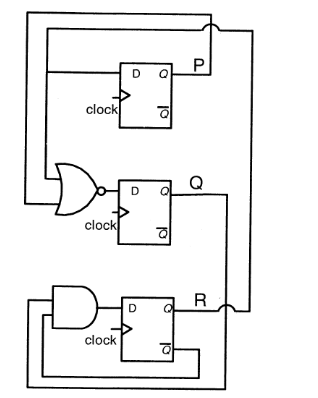
\includegraphics[width=0.3\linewidth]{figs/fig9.png}
    \caption{ }
    \label{fig9}
\end{figure}
\item If at some instance prior to the occurrence of the clock edge, $P, Q$ and $R$ have a value $0, 1$ and $0$ respectively, what shall be the value of $PQR$ after the clock edge? \hfill \textbf{(GATE EE 2025)}

\begin{enumerate}
\begin{multicols}{4}
    \item 000
    \item 001
    \item 010
    \item 011
    \end{multicols}
\end{enumerate}


\item If all the flip-flops were reset to $0$ at power on, what is the total number of distinct outputs (states) represented by $PQR$ generated by the counter? \hfill \textbf{(GATE EE 2025)}

\begin{enumerate}
\begin{multicols}{4}
    \item 3
    \item 4
    \item 5
    \item 6
    \end{multicols}
\end{enumerate}

\textbf{Linked Answer Questions}

\textbf{Statement for Linked Answer Questions 52 and 53:}\\
Consider a network with five nodes, N1 to N5, as shown below.


The network uses a Distance Vector Routing protocol. Once the routes have stabilized, the distance vectors at different nodes are as following.
\begin{figure}[h]
    \centering
    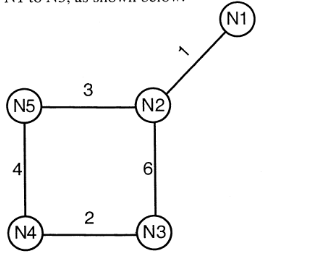
\includegraphics[width=0.5\linewidth]{figs/fig10.png}
    \caption{}
    \label{fig10}
\end{figure}

\[
\begin{aligned}
N1 &: (0, 1, 7, 8, 4) \\
N2 &: (1, 0, 6, 7, 3) \\
N3 &: (7, 6, 0, 2, 6) \\
N4 &: (8, 7, 2, 0, 4) \\
N5 &: (4, 3, 6, 4, 0)
\end{aligned}
\]

Each distance vector is the distance of the best known path at that instance to nodes N1 to N5, where the distance to itself is $0$. Also, all links are symmetric and the cost is identical in both directions. In each round, all nodes exchange their distance vectors with their respective neighbors. Then all nodes update their distance vectors. In between two rounds, any change in cost of a link will cause the two incident nodes to change only that entry in their distance vectors.


\item The cost of link $N_2-N_3$reduces to $2$ (in both directions). After the next round of updates, what will be the new distance vector at node N3? \hfill \textbf{(GATE EE 2025)}

\begin{enumerate}
\begin{multicols}{4}
    \item $\brak{3, 2, 0, 2, 5}$
    \item $\brak{3, 2, 0, 2, 6}$
    \item $\brak{7, 2, 0, 2, 5}$
    \item $\brak{7, 2, 0, 2, 6}$
    \end{multicols}
\end{enumerate}


\item After the update in the previous question, the link $N1-N2$ goes down. N2 will reflect this change immediately in its distance vector as cost $\infty$. After the \textbf{next round of update}, what will be the cost to N1 in the distance vector of N3?\hfill \textbf{(GATE EE 2025)}

\begin{enumerate}
\begin{multicols}{4}
    \item $3$
    \item $9$
    \item $10$
    \item $\infty$
    \end{multicols}
\end{enumerate}
\textbf{Statement for Linked Answer Questions 54 and 55}
An undirected graph G\brak{V,E} contains n \brak{n>2} nodes named $v_1,v_2,.....,v_n$.Two nodes $v_i,v_j$ are connected if and only if $0<|i-j| \leq 2$. Each edge $\brak{v_1,v_2}$is assigned a weight $i+j$.A sample graph with $n=4$ is shown below.
\begin{figure}[h]
    \centering
    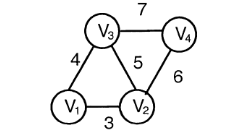
\includegraphics[width=0.5\linewidth]{figs/fig11.png}
    \caption{ }
    \label{fig11}
\end{figure}
\item What will the cost of the minimum spanning tree(MST) of such a graph with n nodes?\hfill \textbf{(GATE EE 2025)}
\begin{enumerate}
 \begin{multicols}{4}
     \item   $\frac{1}{12}\brak{11n^2-5n}$
     \item $n^2-n+1$
     \item $6n-11$
     \item $2n+1$
     \end{multicols}
   
\end{enumerate}
\item The length of the path from $v_5$ to $v_6$ in the MST of the previous question with $n=10$ is \hfill \textbf{(GATE EE 2025)}
\begin{enumerate}
\begin{multicols}{4}
    \item $11$
    \item $25$
    \item $31$
    \item $41$
    \end{multicols}
\end{enumerate}
\textbf{General aptitude \brak{GA} Questions}
\\
\textbf{Q56-Q60 carry one mark each}
\item  Which of the following options is the closest in meaning to the word below: \\\textbf{inexpensible} \hfill \textbf{(GATE EE 2025)}

\begin{enumerate}
    \item Incomprehensible
    \item Indelible
    \item Inextricable
    \item Infallible
\end{enumerate}
\item  If $\log_e (P) =(\frac{1}{2}) \log_(Q)=(\frac{1}{3}) \log_e (R)$, then which of the following options is \textbf{TRUE}? \hfill \textbf{(GATE EE 2025)}
\begin{enumerate}
    \begin{multicols}{4}
        \item $p^2=Q^3 R^2$
        \item $Q^2=PR$
        \item $Q^2=R^3 P$
        \item $R=P^2Q^2$
    \end{multicols}
\end{enumerate}
\item  Choose the most appropriate words from the options given below to complete the following sentence:

\textbf{I contemplated \underline{\makebox[2cm]{\hfill}} for my vacation but decided against it.} \hfill \textbf{(GATE EE 2025)}

\begin{enumerate}
    \item to visit India
    \item visiting to India
    \item to visit
    \item visit to
\end{enumerate}
\item Choose the most appropriate word from the options given below to complete the following sentence.\\
\textbf{If you are trying to make a strong impression on your audience,you cannot do so by being understand ,tentative or \underline{\makebox[2cm]{\hfill}} } \hfill \textbf{(GATE EE 2025)}
\begin{enumerate}
    \item hyperbolic
    \item restrained
    \item argumentative
    \item indifferent
\end{enumerate}
\item Choose the word from the options given below that is most nearly opposite in meaning to the given word: \\
\textbf{Amalgamate} \hfill \textbf{(GATE EE 2025)}
\begin{enumerate}
    \item merge
    \item split
    \item collect
    \item separate
\end{enumerate}
\textbf{Q60 to Q65 carry 2 marks each}
\item  \textbf{Few school curricula include a unit on how to deal with bereavement and grief, and yet all students at some point in their lives suffer from losses through death and parting.} 

Based on the above passage, which topic would not be included in a unit on bereavement?  \hfill \textbf{(GATE EE 2025)}
\begin{enumerate}
    \item how to write a letter of condolence
    \item what emotional stages are passed through in the healing process
    \item what the leading causes of death are
    \item how to give support to a grieving friend
\end{enumerate}
\item  P, Q, R and S are four types of dangerous microbes recently found in a human habitat. The area of each circle with its diameter printed in brackets represents the growth of a single microbe surviving the human immunity system within 24 hours of entering the body. The danger to human beings varies proportionately with the toxicity, potency and growth attributed to a microbe shown in the figure below:
\begin{figure}[H]
    \centering
    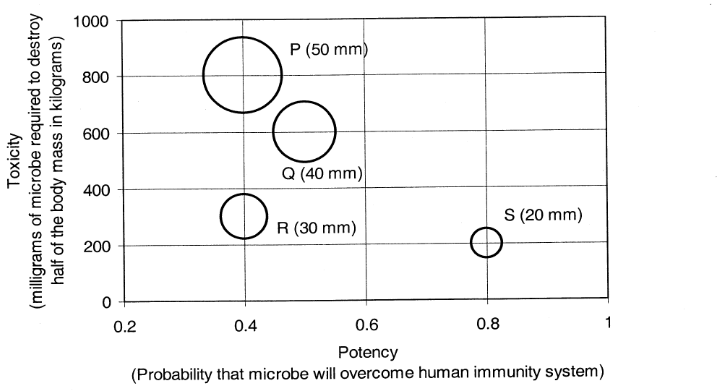
\includegraphics[width=0.6\linewidth]{figs/fig12.png}
    \caption{ }
    \label{fig12}
\end{figure}
A pharmaceutical company is contemplating the development of a vaccine against the most dangerous microbe. Which microbe should the company target in its first attempt? \hfill \textbf{(GATE EE 2025)}
\begin{enumerate}
    \item P
    \item Q
    \item R
    \item S
\end{enumerate}
\item  The variable cost ($V$) of manufacturing a product varies according to the equation $V = 4q$, where $q$ is the quantity produced. The fixed cost ($F$) of production of the same product reduces with $q$ according to the equation $F = \frac{100}{q}$. How many units should be produced to minimize the total cost ($V+F$)? \hfill \textbf{(GATE EE 2025)}  
\begin{enumerate}
\begin{multicols}{4}
    \item 5
    \item 4
    \item 7
    \item 6
    \end{multicols}
\end{enumerate}
\item  A transporter receives the same number of orders each day. Currently, he has some pending orders (backlog) to be shipped. If he uses 7 trucks, then at the end of the 4th day he can clear all the orders. Alternatively, if he uses only 3 trucks, then all the orders are cleared at the end of the 10th day. What is the minimum number of trucks required so that there will be no pending order at the end of the 5th day? \hfill \textbf{(GATE EE 2025)}  
\begin{enumerate}
\begin{multicols}{4}
    \item $4$
    \item $5$
    \item $6$
    \item $7$
    \end{multicols}
\end{enumerate}
\item  A container originally contains 10 litres of pure spirit. From this container 1 litre of spirit is replaced with 1 litre of water. Subsequently, 1 litre of the mixture is again replaced with 1 litre of water and this process is repeated one more time. How much spirit is now left in the container?  \hfill \textbf{(GATE EE 2025)} 
\begin{enumerate}
\begin{multicols}{4}
    \item $7.58 \text{litres}$
    \item $7.84 \text{litres}$
    \item $7 \text{litres}$
    \item $7.29 \text{litres}$
    \end{multicols}
\end{enumerate}
\end{enumerate}
\end{document}
